
\subsection{Setting the number of ICs}

After having undergone the initial standard preprocessing presented in \secref{Standardpre}, the next step was to extract the independent components (IC) using MELODIC. But before the data could be subjected to the ICA, several considerations were made in order to increase ICA performance. The separation of sources is highly dependent on the number of ICs (N-ICs) chosen and therefore crucial for the FIX end performance. Consequently an investigation of the optimal number of components was conducted. The risk of underestimating the number of components, would result in a loss of information and suboptimal signal extraction \cite{Beckmann2004}. Contrary, overestimating the number of components would result in a false representation, as the different informative sources would be split leaving fractional sources, which would be very hard to identify and utilize \cite{Beckmann2004,Li2007}. \\
Data used for investigating the optimal number of components was derived from ten randomly chosen subjects having three heat runs each. This made for 30 IC analyses each completed utilizing the MELODIC tool. 


\subsubsection{Default mode}
Initially no limit was selected and the MELODIC algorithm per default estimated the optimal number of components, as recommended by the MELODIC developers. \cite{FMRIB2016} The MELODIC tool provided analyses with the estimated number of component to represent the variance ranging from 9-64 components. Due to the substantial amount of variability in the number of components estimated, the degree to how much the sources had been separated varied substantially between the components. Inspecting the output from the ICA, which produced nine components, it became clear that the separation of sources was not sufficient, as the components was mixtures of multiple sources of noise and signal. Furthermore no task related activation where seen in any of the components indicating that variance of noise accounted for the first nine components. Inspecting the analyses with the highest number of components, it became evident that the algorithm had overestimated the number of ICs, leaving empty and fractured activation in the components unrecognizable for labeling. Because of the MELODIC ICA on default mode overestimating and underestimating the number of components, a case specific analysis for the optimal number of components was conducted. 

\subsubsection{N-IC analysis}

Seeking guidelines in the literature, various articles have worked with estimating the optimal number of components. In the case of Majeed et al. \cite{Majeed2014}, results indicate that a N-IC lower than 5 components would lead to an underestimation and more than 50 components would result in overestimation. The optimal N-IC was found to be 10. Another study limited the number of components to 20 as this was found to preserve much of the information without overestimating \cite{Calhoun2001} Furthermore other studies limited the number to 25 components \cite{Kim2013,Erpelding2013}. Building on this knowledge, MELODIC was run on the ten subjects again limiting the N-ICs to 15, 20, 25, 30 to assess which would give the optimal separation between signal and noise, and in separating the independent sources for each. The assessment was made by counting the following outcomes: 
\begin{itemize}
	\item The number of components containing signal activation from multiple sources or unrecognizable due to fragmentation. 
	\item The number of components containing signal activation from a single source 
	\item The number of components containing no activation    
\end{itemize}
 
Examples of spatial maps containing multiple sources, fragmented sources and a single source can be seen in \figref{fig:meth:Unknown}, \figref{fig:meth:Frag} and \figref{fig:meth:Movement}, respectively. Identification of sources was supported by utilizing the guidelines presented in \cite{Griffanti2017}, showing how the different noise sources would be present in the spatial map and using the information of which brain regions would be activated during pain stimuli as presented in \secref{sec:pain}. Both investigators conducted the assessment. One found 25 components to be optimal, whilst the other found that 30 components was more favorable. The assessment was assisted by incorporating consulting from an expert on the area. With help from experts advice, 25 components was identified to provide the best separation of sources in the data. This decision was well supported by the results of the prior studies of \cite{Kim2013,Erpelding2013}.     

\begin{figure}[H]                 
	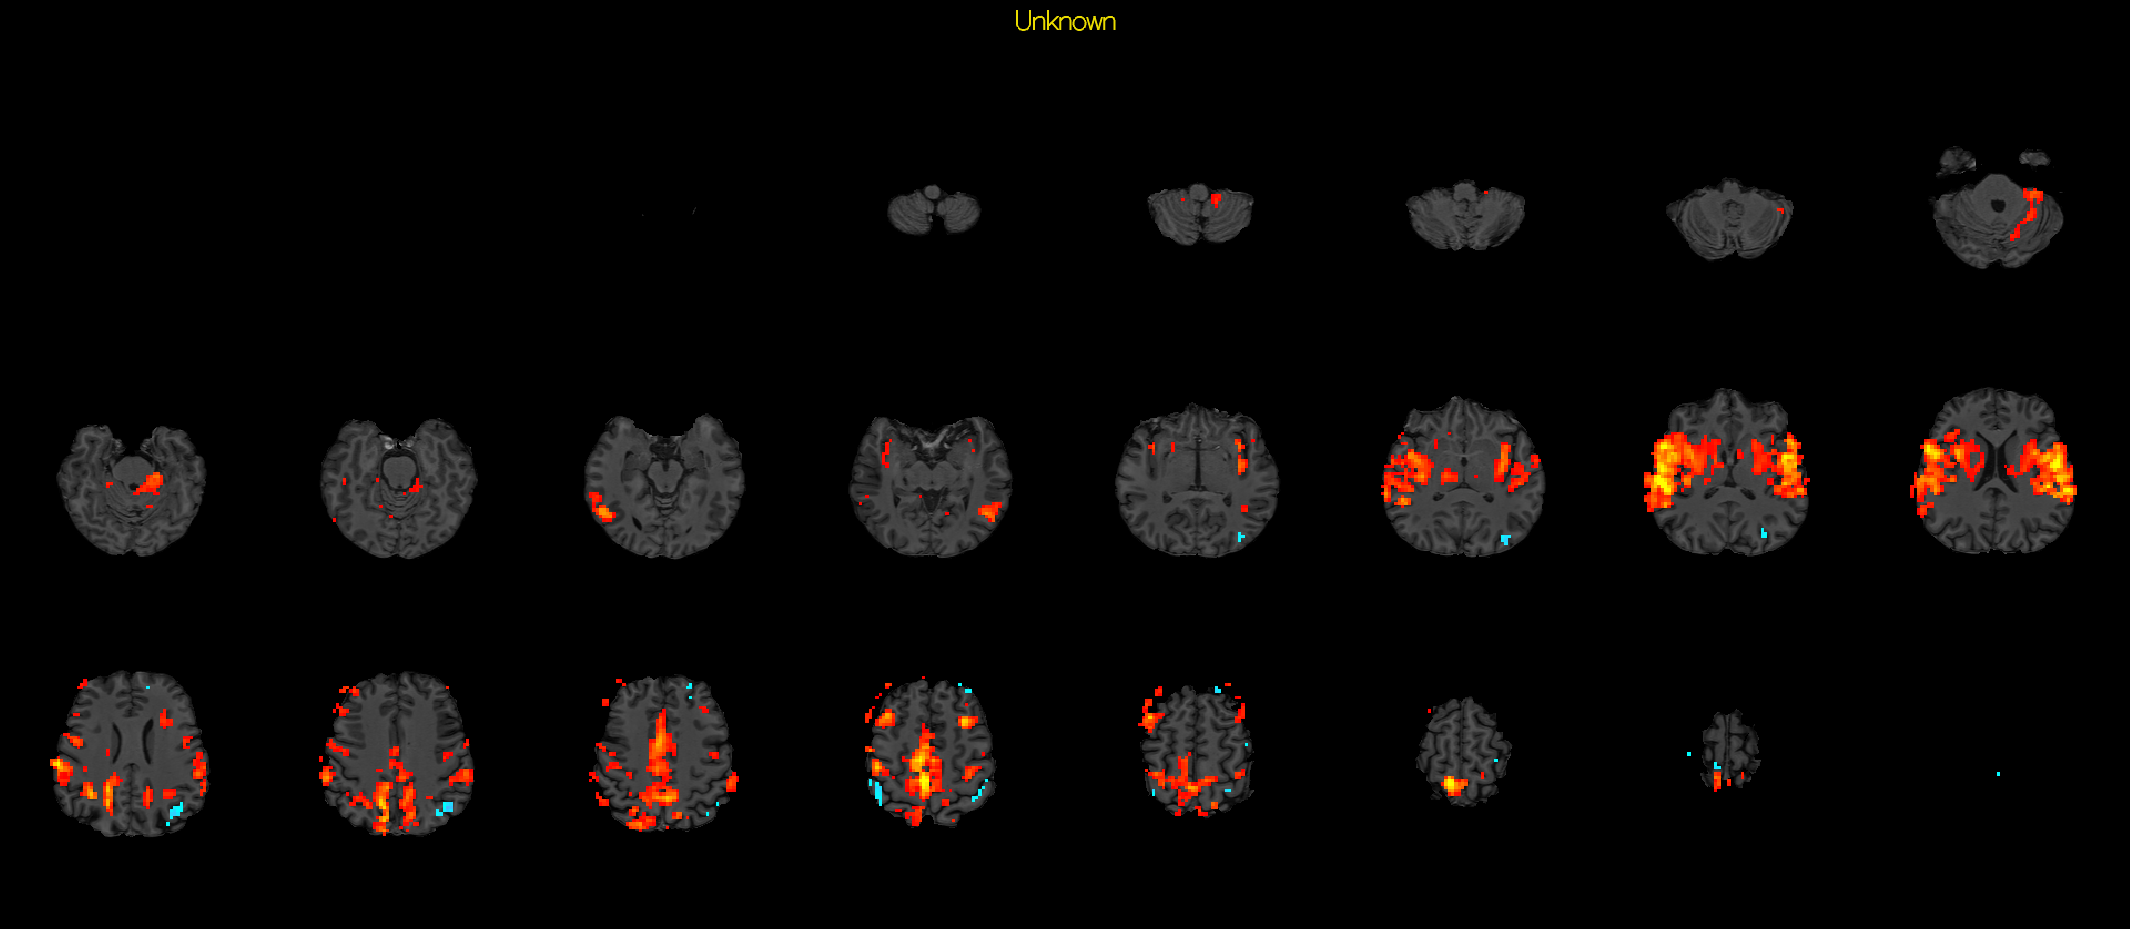
\includegraphics[width=.8\textwidth]{figures/bMethods/Unknown}  
	\caption{An example of a  component with a spatial map for a component showing activation from multiple sources. Activation cannot be localized to single brain regions.}
	\label{fig:meth:Unknown} 
\end{figure}

\begin{figure}[H]                 
	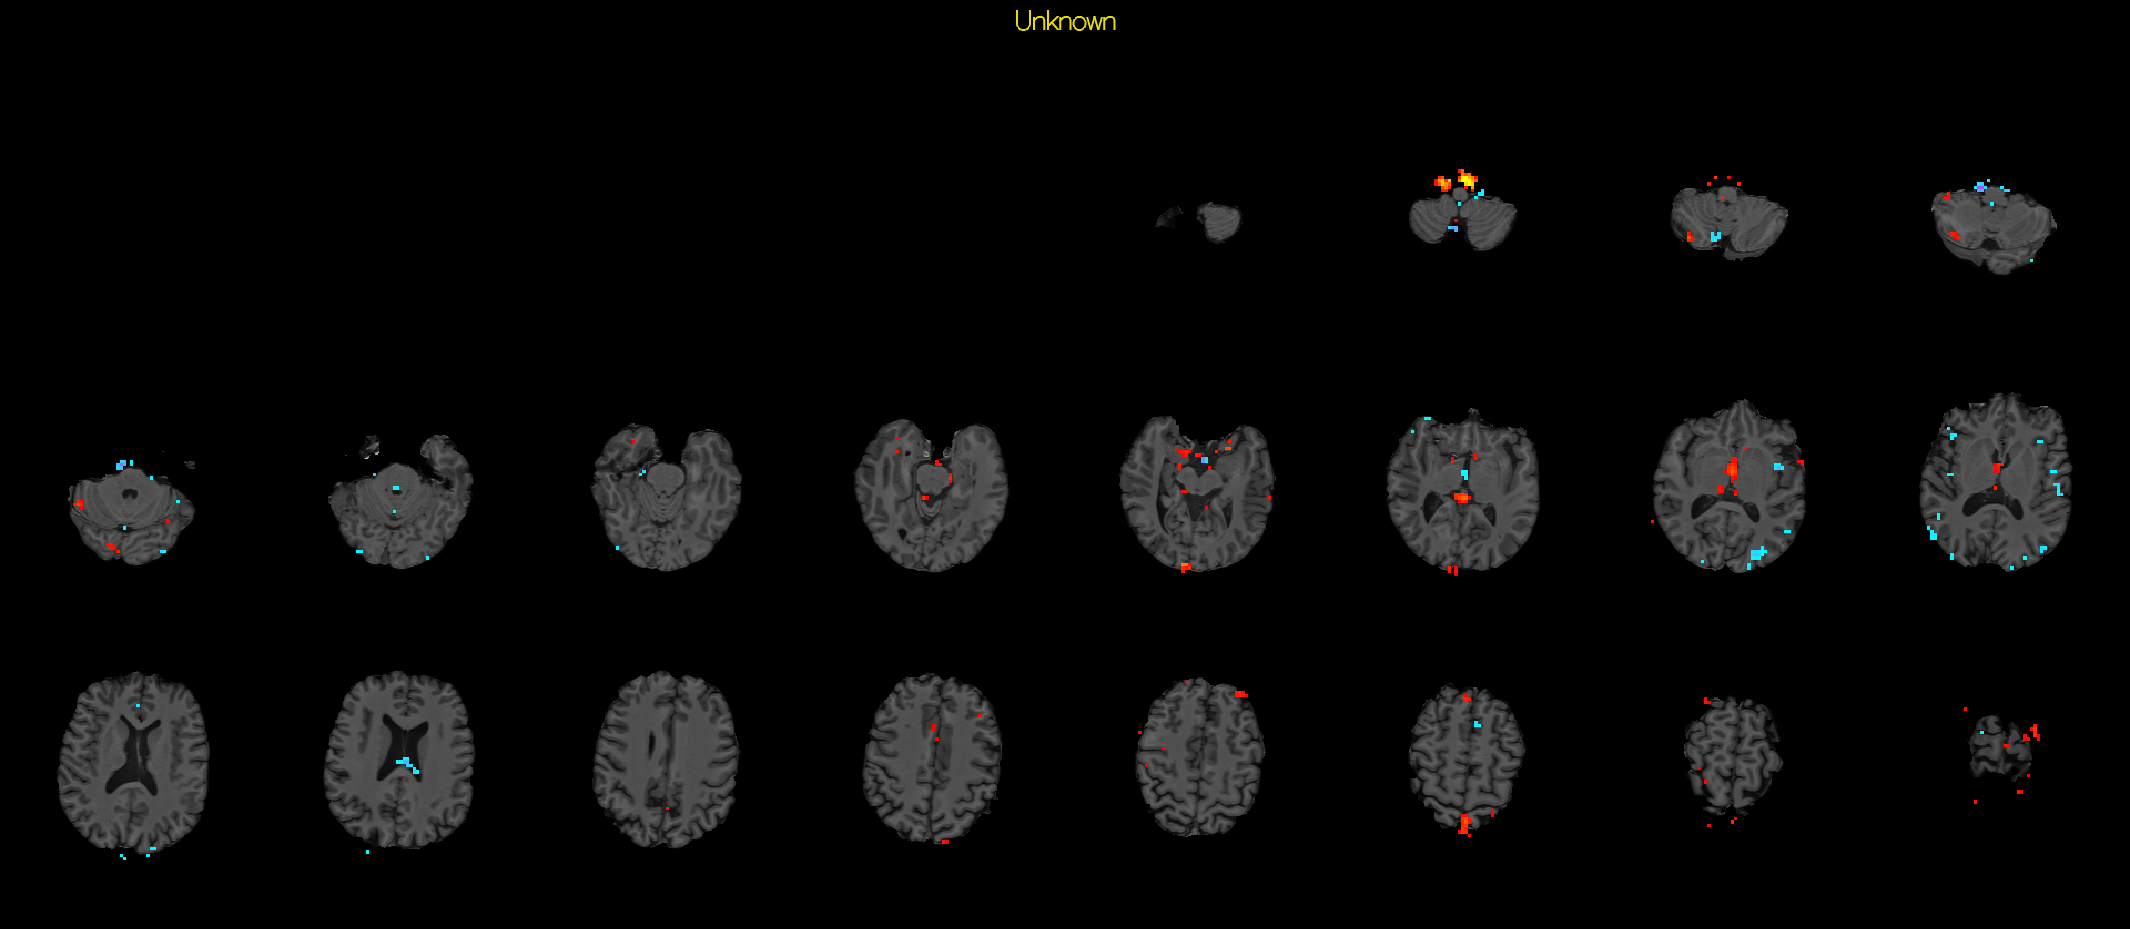
\includegraphics[width=.8\textwidth]{figures/bMethods/Frag}  
	\caption{An example of a component with a fragmented spatial map illustrating that no brain activation or artifactual noise can localized.}
	\label{fig:meth:Frag} 
\end{figure}

\begin{figure}[H]                 
	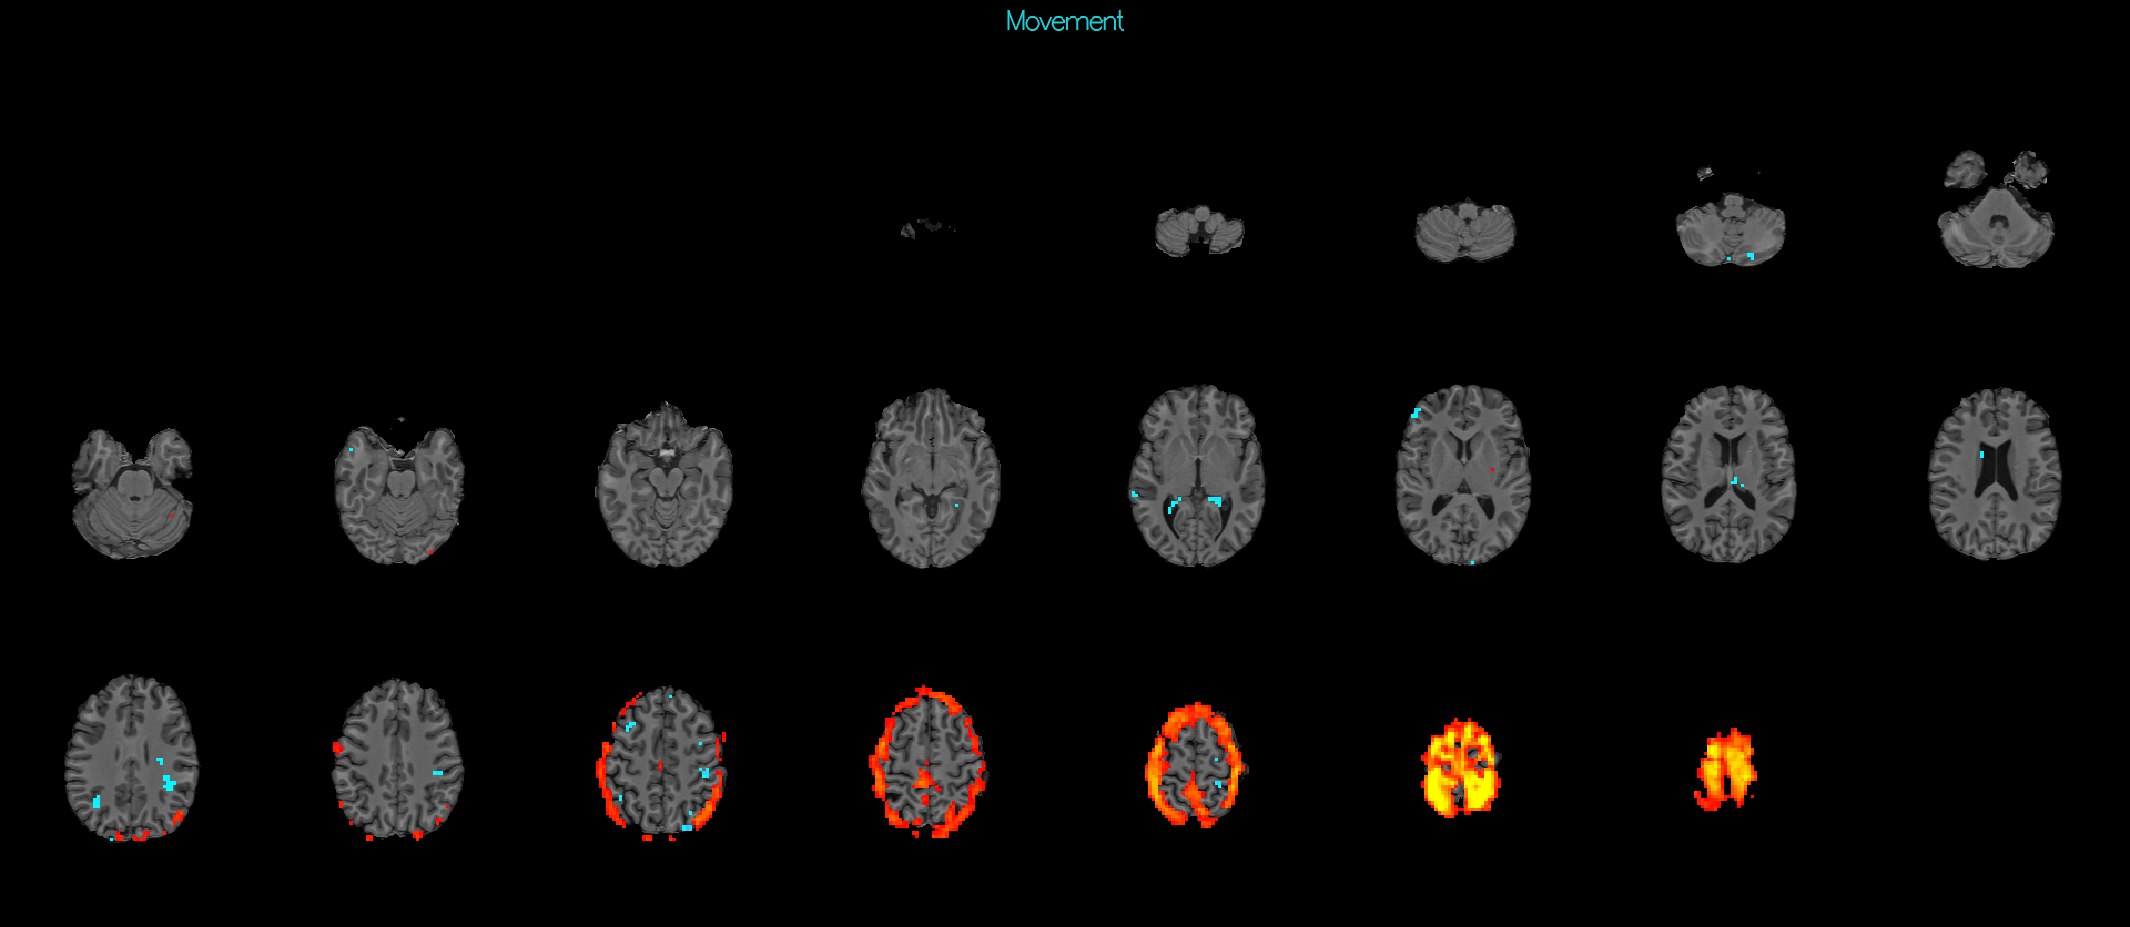
\includegraphics[width=.8\textwidth]{figures/bMethods/Movement}  
	\caption{An example of a spatial map showing a clearly recognizable artifact in the form of movement dominating the component.}
	\label{fig:meth:Movement} 
\end{figure}






 